\documentclass[a4paper,10pt]{article}
\usepackage[utf8]{inputenc}
\usepackage{amsmath}
\usepackage{amsfonts}
\usepackage{amssymb}
\usepackage{algorithm}
\usepackage[noend]{algpseudocode}
\usepackage{program}
\usepackage{amsmath}
\usepackage{graphicx}
\usepackage[T1]{fontenc}
\usepackage{eso-pic}
%\usepackage{gensymb}
\usepackage{listings}
\usepackage{float}

\usepackage{xcolor}
\definecolor{alternateKeywordsColor}{rgb}{0.13,1,0.13}
\definecolor{keywordsColor}{rgb}{0.13,0.13,1}
%\definecolor{commentsColor}{rgb}{0,0.5,0}
\definecolor{commentsColor}{rgb}{0,0.5,0}
%\definecolor{stringsColor}{rgb}{0.9,0,0}
\definecolor{stringsColor}{rgb}{0,0,0.5}
\definecolor{light-gray}{gray}{0.95}

\lstdefinelanguage{fsharp}{%
  keywords={abstract, and, as, assert, base, begin, class, default, delegate, do, done, downcast, downto, elif, else, end, exception, extern, false, finally, for, fun, function, global, if, in, inherit, inline, interface, internal, lazy, let, match, member, module, mutable, namespace, new, null, of, open, or, override, private, public, rec, return, sig, static, struct, then, to, true, try, type, upcast, use, val, void, when, while, with, yield},
  morekeywords={atomic, break, checked, component, const, constraint, constructor, continue, eager, fixed, fori, functor, include, measure, method, mixin, object, parallel, params, process, protected, pure, recursive, sealed, tailcall, trait, virtual, volatile},
  otherkeywords={ let!, return!, do!, yield!, use!},
  keywordstyle=\color{keywordsColor},
  %sensitive=true,
  basicstyle=\ttfamily\lst@ifdisplaystyle\small\fi, % make font small for listings but not for lstinline
  breaklines=true,
  morecomment=[l][\color{commentsColor}]{///},
  morecomment=[l][\color{commentsColor}]{//},
  morecomment=[s][\color{commentsColor}]{{(*}{*)}},
  morestring=[b]",
  showstringspaces=false,
  literate={`}{\`}1,
  stringstyle=\color{stringsColor},
  %aboveskip=0pt, 
  %belowskip=0pt,
  %resetmargins=true,
  captionpos=b,
  backgroundcolor=\color{black!5!white},
}
\lstdefinelanguage{ebnf}{%
  keywords={},
  morekeywords={},
  otherkeywords={},
  keywordstyle=\color{keywordsColor},
  % sensitive=true,
   basicstyle=\fontfamily{pcr}\selectfont\lst@ifdisplaystyle\small\fi, 
   breaklines=true,
  morecomment=[s][\color{commentsColor}]{{(*}{*)}},
  morestring=[b]",
  morestring=[b]',
  alsoletter={\\},
  showstringspaces=false,
  %stringstyle=\color{stringsColor},
  %aboveskip=0pt, 
  %belowskip=0pt,
  %resetmargins=true,
  captionpos=b,
  backgroundcolor=\color{blue!10!white},
}
\lstdefinelanguage{console}{%
  keywords={},
  morekeywords={},
  otherkeywords={},
  basicstyle=\ttfamily\lst@ifdisplaystyle\small\fi, 
  breaklines=true,
  showstringspaces=false,
  % aboveskip=0pt, 
  % belowskip=0pt,
  %resetmargins=true,
  captionpos=b,
  backgroundcolor=\color{green!10!white},
}
\lstset{language=fsharp, frame=single}
\usepackage{caption}
\DeclareCaptionStyle{listing} [justification=raggedright,labelfont=bf]{}
\captionsetup[lstlisting]{style=listing}


\newcommand\floor[1]{\lfloor#1\rfloor}
\newcommand\ceil[1]{\lceil#1\rceil}
\newcommand{\BackgroundPic}{\put(-4,0){\parbox[b][\paperheight]{\paperwidth}{\centering
\includegraphics[width=\paperwidth,height=\paperheight]{nat-farve.pdf}}}}

\algnewcommand\True{\textbf{true}\space}
\algnewcommand\False{\textbf{false}\space}
\algdef{SE}[SUBALG]{Indent}{EndIndent}{}{\algorithmicend\ }%
\algtext*{Indent}
\algtext*{EndIndent}

\begin{document} 
	\AddToShipoutPicture*{\BackgroundPic}
	
	\begin{titlepage}
		\thispagestyle{empty}
		\vspace*{5cm}
		\begin{center}
			\Huge \textbf{Programmering og Problemløsning} \\
			\LARGE \textbf{Aflevering 12i} \\
		\end{center}
		\vspace*{3.5cm}
		\begin{flushleft}
			
		\begin{table}[h!]
			\begin{tabular}{lll}
				Adam Ingwersen\\
			\end{tabular}
		\end{table}
			
			
			\vspace{3mm}
			\vspace{3mm}
			Datalogisk  Institut\\
			Københavns Universitet\\
			\vspace{3mm}
			\today\\
			%\vspace*{0.5cm}
			
		\end{flushleft}
	\end{titlepage}

	\title{10g}
	\author{AAP}
	
	\newpage
\newpage
\section{Programbeskrivelse}
Hensigten med programmet har været, at lave et visualiseringsprogram, der lader brugeren vælge et billede samt udformningen af et dertilhørende gråtone-histogram. Progammetbeskrivelsen deles op i 3 sektioner:

\subsection{Brugerinteraktion}
Fsharp's \texttt{Text.RegularExpressions} samt \texttt{IO} namespaces anvendes her til at liste forskellige jpg-filer indeholdt af programfolderen i konsollen. Hertil promptes brugeren til at vælge et af billederne. Brugeren promptes ligeledes for valg af antal bins i histogrammet - mellem 1 og 1200; inputtet lagres i den mutérbare variabel \texttt{noBins}. Brugeren har mulighed for at vælge 2 forskellige skaleringer af histogrammet; inputtet lagres i \texttt{scales}. 
Brugerens input samles med en tekststreng således at den ønskede fil importeres med \texttt{Image.fromFile}\footnote{Alle funktioner med "Image" er fra Jon Sporrings \texttt{image.fs}-modul som er vedlagt afleveringen.}. Det indlæste billedfil konverteres til gråtoner med \texttt{Image.toGray}, hvorefter der dannes et gråtonehistogram vha. \texttt{Image.histogram}.

\subsection{Koordinater}
Winforms skal bruge input af typen \texttt{Point()} til dannelse af en billedfil. Udfordringen her, har været, at lade disse koordinater blive dannet dynamisk i relation til hinanden - samtidigt med at kunne bliver skaleret. Funktionen \texttt{makeColumnList} har 4 konstruktorer; et float-array og et int-array, som \texttt{Image.histogram} returnerer, samt antallet af bins(bøtter) og en skaleringsfaktor. Funktionen appender herfra hver enkelt bin, bestående af 4 punkter til \texttt{columnList}. Disse punkter er determineret via et 1) if/else statement og 2) den foregående bins position på x-aksen. If/else statementet sikrer, at den allerførste bin, der skal bestemmes bliver bestemt absolut - ikke relativt til den foregående bin. Ellers, genereres et sæt af punkter, relativt til de foregående. X-koordinaterne bestemmes vha. en afstand-konstant (denne er predefineret udenfor funktionen, men afhænger af antallet af bins), samt x-koordinaterne for den umiddelbare forrige bin. Y-koordinaterne determineres ud fra den højeste y-værdi samt skaleringsparametren. 

Desuden konstrueres x- og y-akserne uden for funktionen. 

\subsection{Visualisering}
Med punkterne på plads, laves en tegne-funktion, \texttt{drawColumns}. Her bruges en \texttt{pen} til at tegne streger mellem punkterne samt en \texttt{brush} til at farvelægge hver bin. Dertil laves dynamiske labels; labels ad x-aksen flytter sig relativt til skaleringsfaktoren samt afstands-parametren. Labels ad y-aksen viser varierende tekst relativt til højden af den største bin - her bruges skaleringsfaktoren også.

\section{Evaluering}

Som eksemepel anvendes et billede af et bjerg\footnote{Se Bilag A: Mountain}. Eksemplet viser et gråtone-histogram med 5 bins, hvor det ses, at majoriteten af gråtonerne ligger i det lyse spektrum, ca. halvdelen af observationerne ligger mellem 50-100. Der er meget få observationer i det helt mørke spektrum jf. dette histogram. Ved at vælge f.eks. 100 bins opnås et signifikant mere nuanceret billede af gråtone-fordelingen\footnote{Se Bilag A :Mountain}.

For at teste, at visualiseringen virker efter hensigten, testes programmet mod et billede med meget høje sorte, hhv hvide områder - hvortil det må forventes at fordelingen i histogrammet har noget der minder om en invers normalfordeling (skåleformet)\footnote{Bilag B: Black and White}.

Skulle det ønskes at køre programmet, kan dette gøres vha.:
\begin{lstlisting}{language=console}
	fsharpc -a image.fs && fsharpc -r image.dll 12i0.fsx && mono 12i0.exe
\end{lstlisting}


\newpage

\section*{Bilag}
\subsection*{A: Mountain}

\begin{figure}[H]
  \centering
  \begin{minipage}[b]{0.4\textwidth}
    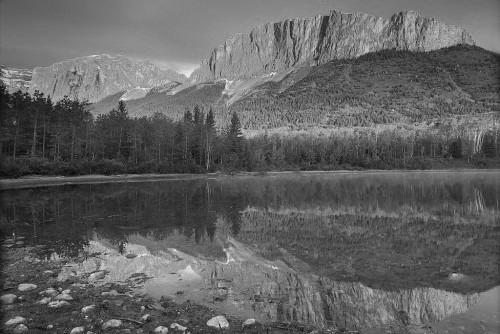
\includegraphics[width=\textwidth]{mountain_gray.jpg}
    \caption{Gråtone billede af bjerglandskab}
  \end{minipage}
  \hfill
  \begin{minipage}[b]{0.4\textwidth}
    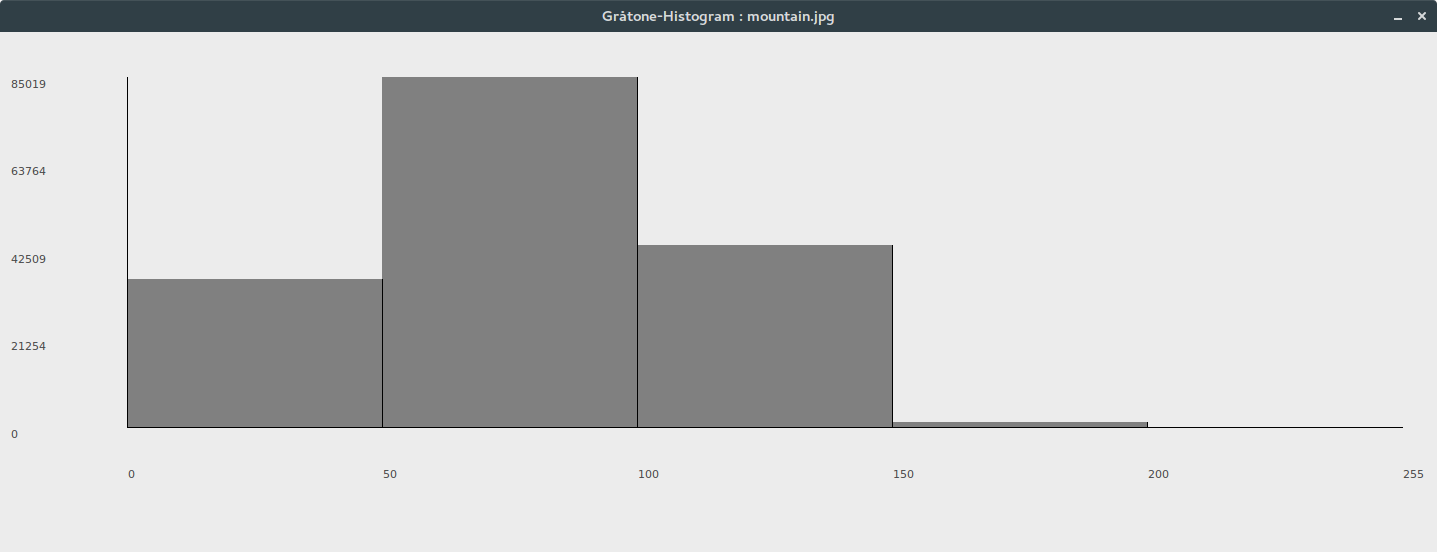
\includegraphics[width=\textwidth]{hist1.png}
    \caption{Gråtone histogram, 5 bins}
  \end{minipage}
\end{figure}

\begin{figure}[H]
	\centering
    	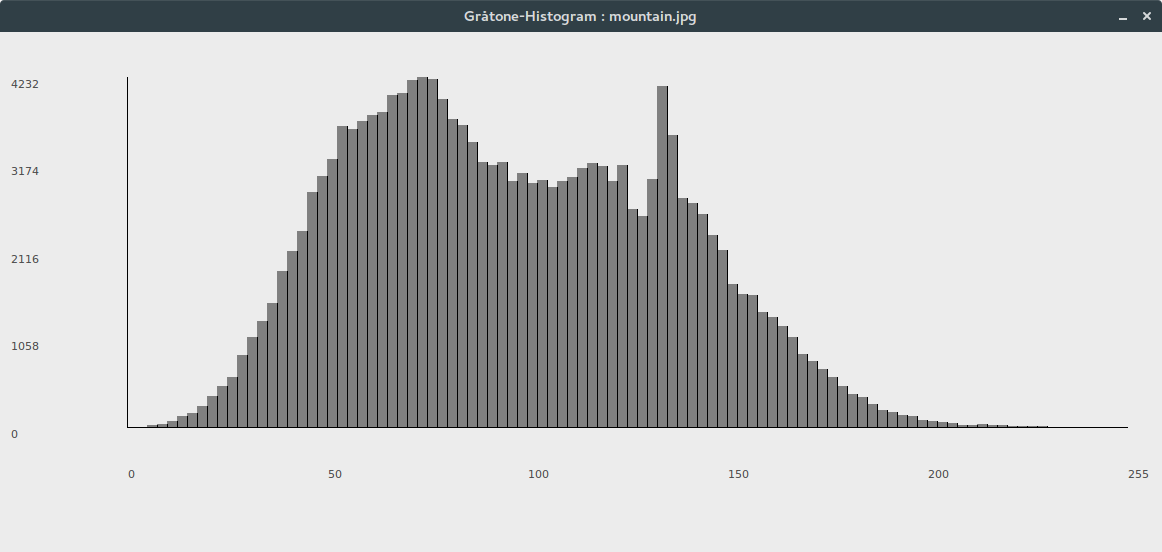
\includegraphics[width=\textwidth]{hist2.png}
    	\caption{Gråtone histogram, 100 bins}
\end{figure}


\subsection*{B: Black and White}

\begin{figure}[H]
  \centering
  \begin{minipage}[b]{0.4\textwidth}
    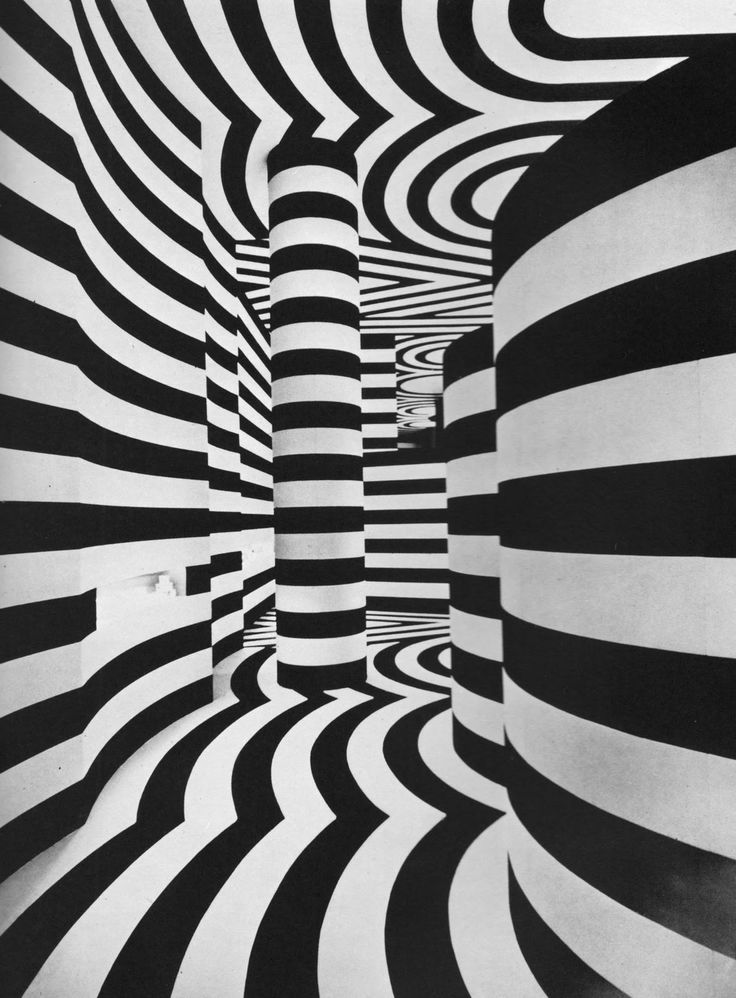
\includegraphics[width=\textwidth]{blackwhite_gray.jpg}
    \caption{Gråtone billede af sort-hvidt rum}
  \end{minipage}
  \hfill
  \begin{minipage}[b]{0.4\textwidth}
    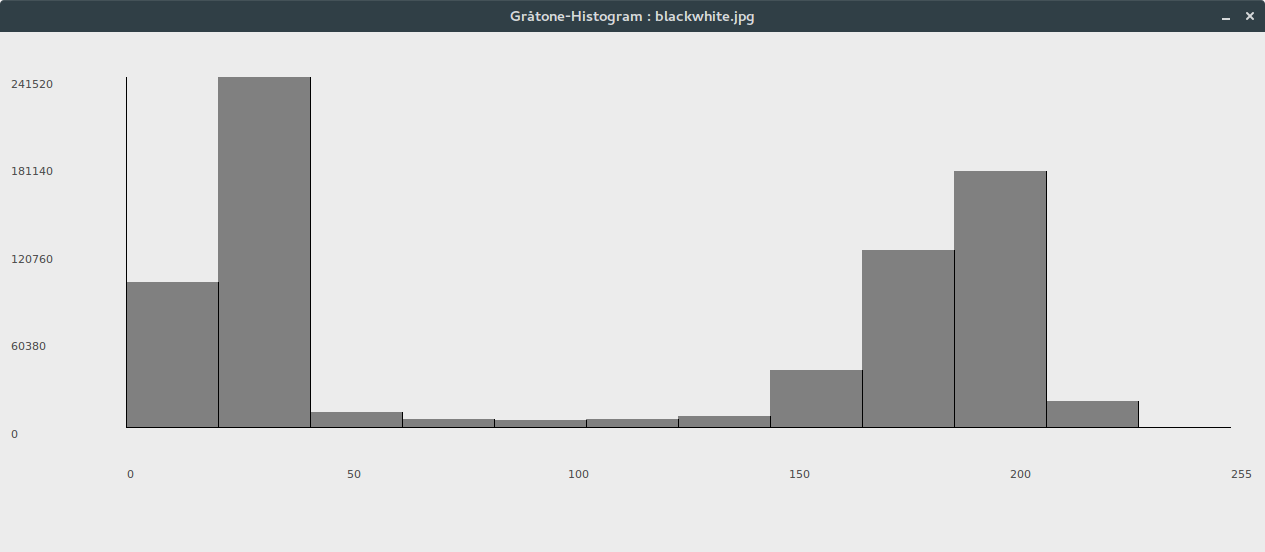
\includegraphics[width=\textwidth]{hist4.png}
    \caption{Gråtone histogram, 12 bins}
  \end{minipage}
\end{figure}

\begin{figure}[H]
	\centering
    	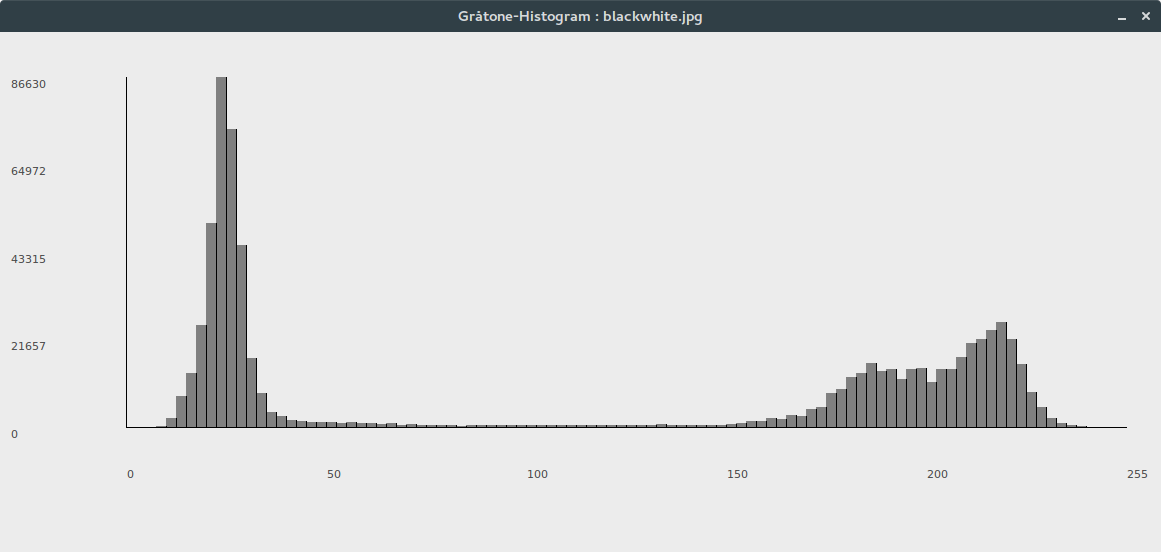
\includegraphics[width=\textwidth]{hist3.png}
    	\caption{Gråtone histogram, 100 bins}
\end{figure}
\end{document}